
%----------------------------------------------------------------------------------------
%	ANALISI DI DEPLOYMENT SU LARGA SCALA
%----------------------------------------------------------------------------------------

\section{Analisi di deployment su larga scala}

L'applicativo è stato progettato tenendo in considerazione la possibilità di essere eseguito su larga scala.\\

\subsection{Client App}
Per quanto riguarda il lato client e il server per l'autenticazione sarebbe possibile eseguire il
deployment su cloud tramite servizi come Vercel \cite{vercel}.\\

Grazie alle funzionalità messe a disposizione dal servizio, è possibile mantenere un deploy
continuo dell'applicativo, in modo da poter aggiornare il codice in produzione in maniera
semplice e veloce, tramite semplici push sul main branch di GitHub \cite{github}, grazie all'integrazione del bot offerto da Vercel.\\

\subsection{Database}
Il deployment del database su un cluster di MongoDB Atlas \cite{atlas} ha svolto un ruolo cruciale nel progetto.
Questa soluzione basata su cloud ha permesso di liberarsi dalla gestione dell'infrastruttura, consentendo
di concentrarsi maggiormente sullo sviluppo dell'applicazione stessa. La scalabilità offerta da MongoDB
Atlas ha garantito prestazioni elevate e adattabilità alle crescenti esigenze dell'applicazione.\\

Inoltre, sono stati sfruttati strumenti avanzati per la sicurezza dei dati e il monitoraggio delle attività.
Complessivamente, questa scelta ha contribuito al successo del progetto, garantendo affidabilità e sicurezza.\\

\subsection{Cluster}
Per quanto riguarda invece il lato "cluster" del sistema, il gruppo ha immaginato di effettuare
il deployment dei ChargingStationActor direttamente nelle stazioni di ricarica, mentre i
componenti Charging Station Provider e Service possono essere deployati su nodi fisicamente
separati dalle stazioni di ricarica. Akka cluster permette al sistema di aggiungere facilmente
nuovi attori di qualunque tipo per soddisfare le esigenze di scalabilità del sistema.\\

Il deployment finale così come immaginato dal gruppo è rappresentato dal seguente diagramma \ref{fig:deployment}:

\begin{figure}[H]
    \centering
    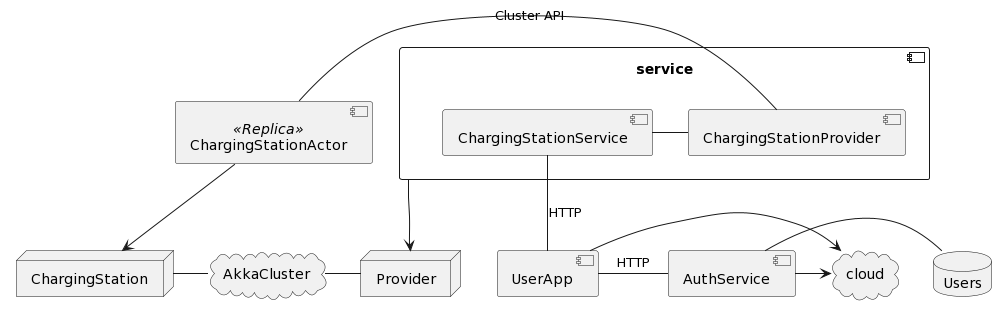
\includegraphics[width=1\textwidth]{images/deployment.png}
    \caption{Diagramma di deployment}
    \label{fig:deployment}
\end{figure}

% In questa sezione va discussa, eventualmente con l'ausilio di opportuni diagrammi (componenti, deployment), l'evoluzione del progetto presentato immaginando che venga adottato su larga scala. I dettagli qui esposti devono quindi astrarre dalle specifiche dell'elaborato qualora l'implementazione sia stata focalizzata su uno scenario isolato.\\

% A titolo d’esempio, qualora applicabile, devono essere evidenziate le criticità che si potrebbero incontrare e devono essere proposte soluzioni tipiche in contesti di \textit{cloud architecture} per garantire un'adeguata \textit{resilienza}, in termini di \textit{availability} e \textit{scalability} del sistema.\\


% Vincoli circa la lunghezza della sezione (escluse didascalie, tabelle, testo nelle immagini, schemi):

% \vspace{1cm}
% \begin{tabular}{l|rr}
%                  & Numero minimo di battute & Numero massimo di battute \\
%     \hline
%     1 componente & 3000                     & 6000                      \\
%     2 componenti & 4500                     & 9000                      \\
%     3 componenti & 6000                     & 12000                     \\
%     \hline
% \end{tabular}


\newpage
